% Template:     Template Reporte LaTeX
% Documento:    Archivo de ejemplo
% Versión:      1.1.7 (04/09/2019)
% Codificación: UTF-8
%
% Autor: Pablo Pizarro R. @ppizarror
%        Facultad de Ciencias Físicas y Matemáticas
%        Universidad de Chile
%        pablo.pizarro@ing.uchile.cl, ppizarror.com
%
% Sitio web:    [https://latex.ppizarror.com/Template-Reporte/]
% Licencia MIT: [https://opensource.org/licenses/MIT]

% ------------------------------------------------------------------------------
% NUEVA SECCIÓN
% ------------------------------------------------------------------------------
% Las secciones se inician con \section, si se quiere una sección sin número se
% pueden usar las funciones \sectionanum (sección sin número) o la función
% \sectionanumnoi para crear el mismo título sin numerar y sin aparecer en el índice

\section{DRAM notes}

This document is intended to be an a simple introduction of how the SDRAM works, look at the main signals of the protocol, explain a little bit how Xilinx FPGA tackles that interface and show how to set the Xilinx MIG. 

%\newp
The basic structure of the DRAMs is just a transistor with a capacitor.
The idea is as follows: When the address of coincidence the transistor gets selected and the word line contains either a high or low value which is the bit that is store in the capacitor. 
To read the procedure is similar, if the address coincide the transistor then a logic element reads the charge inside the capacitor. Note that every time that you read you are erasing the data from the capacitor, so if you change the address that you are reading you have to re-write the data that you read.
Also the capacitor gets discharged over the time, so there should be some logic that refresh each value, that's why this types of memory are called dynamic. 



\begin{figure}
    \centering
    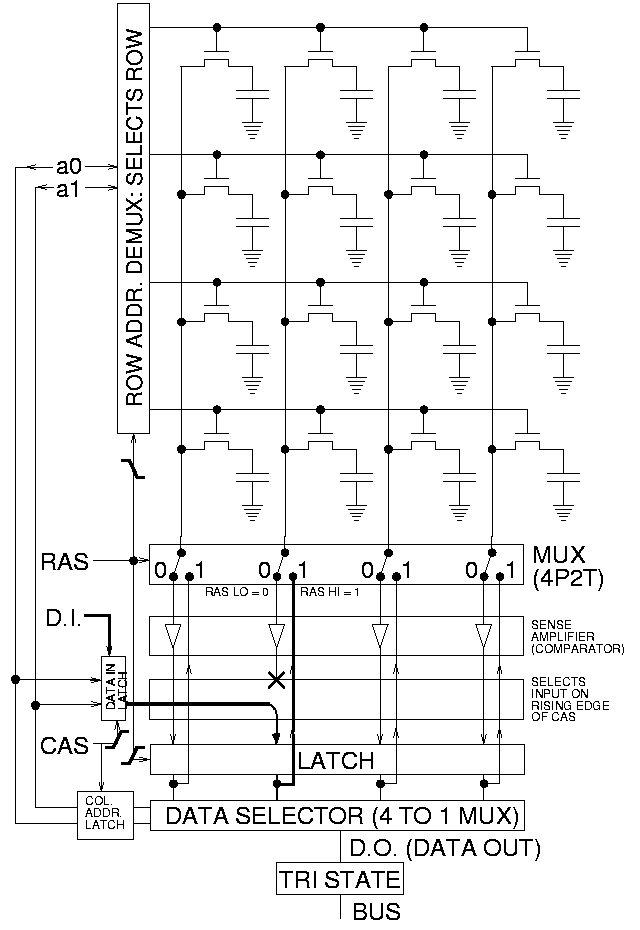
\includegraphics[scale=0.3]{img/dram.png}
    \caption{Basic DRAM diagram}
    \label{fig:dram_diag}
\end{figure}

%\newp 
The diagram of the DRAM in \ref{fig:dram_diag} consists in two indices, the row and the column. When you select a row the data gets read and charged into a row buffer, then you read the data using the column address.

The idea is that if you later try to read a column in the same row you don't have to go to the memory itself to obtain the data, it already in the buffer. 

There are three main commands to read or write values in the DRAM:

\begin{itemize}
    \item \textbf{Activate}:Open the selected row and place it into the row buffer.
    \item \textbf{Read/Write}: Read or write the column value.
    \item \textbf{Precharge}: Re-write the data into the column.
\end{itemize}

If the row is already open you just have to read/write the data, if there is a request for a closed row you have to pay and write the data into the row, then move the data from the correspondent address to the row buffer and then you could read it.
So in this case the best is to open a row a write/read the columns in this row before change to another one.

%\newp
\section{DRAM Hierarchy}

The DRAM has a hierarchical architecture:
\begin{itemize}
    \item Dual in line memory module (DIMM) is the typical RAM module in computers that everybody has in his mind. Most DIMMs are built using "×4" or "×8" memory chips with nine or eight chips per side where the number refer to the data width of the DRAM chips in bits. For example x4 means that the data width per side is 36 in each side.  
    
    There are a lot of variation of the DIMMs, like for example the SODIMM which is a Small Outline DIMM.
    
    \begin{figure}
        \centering
        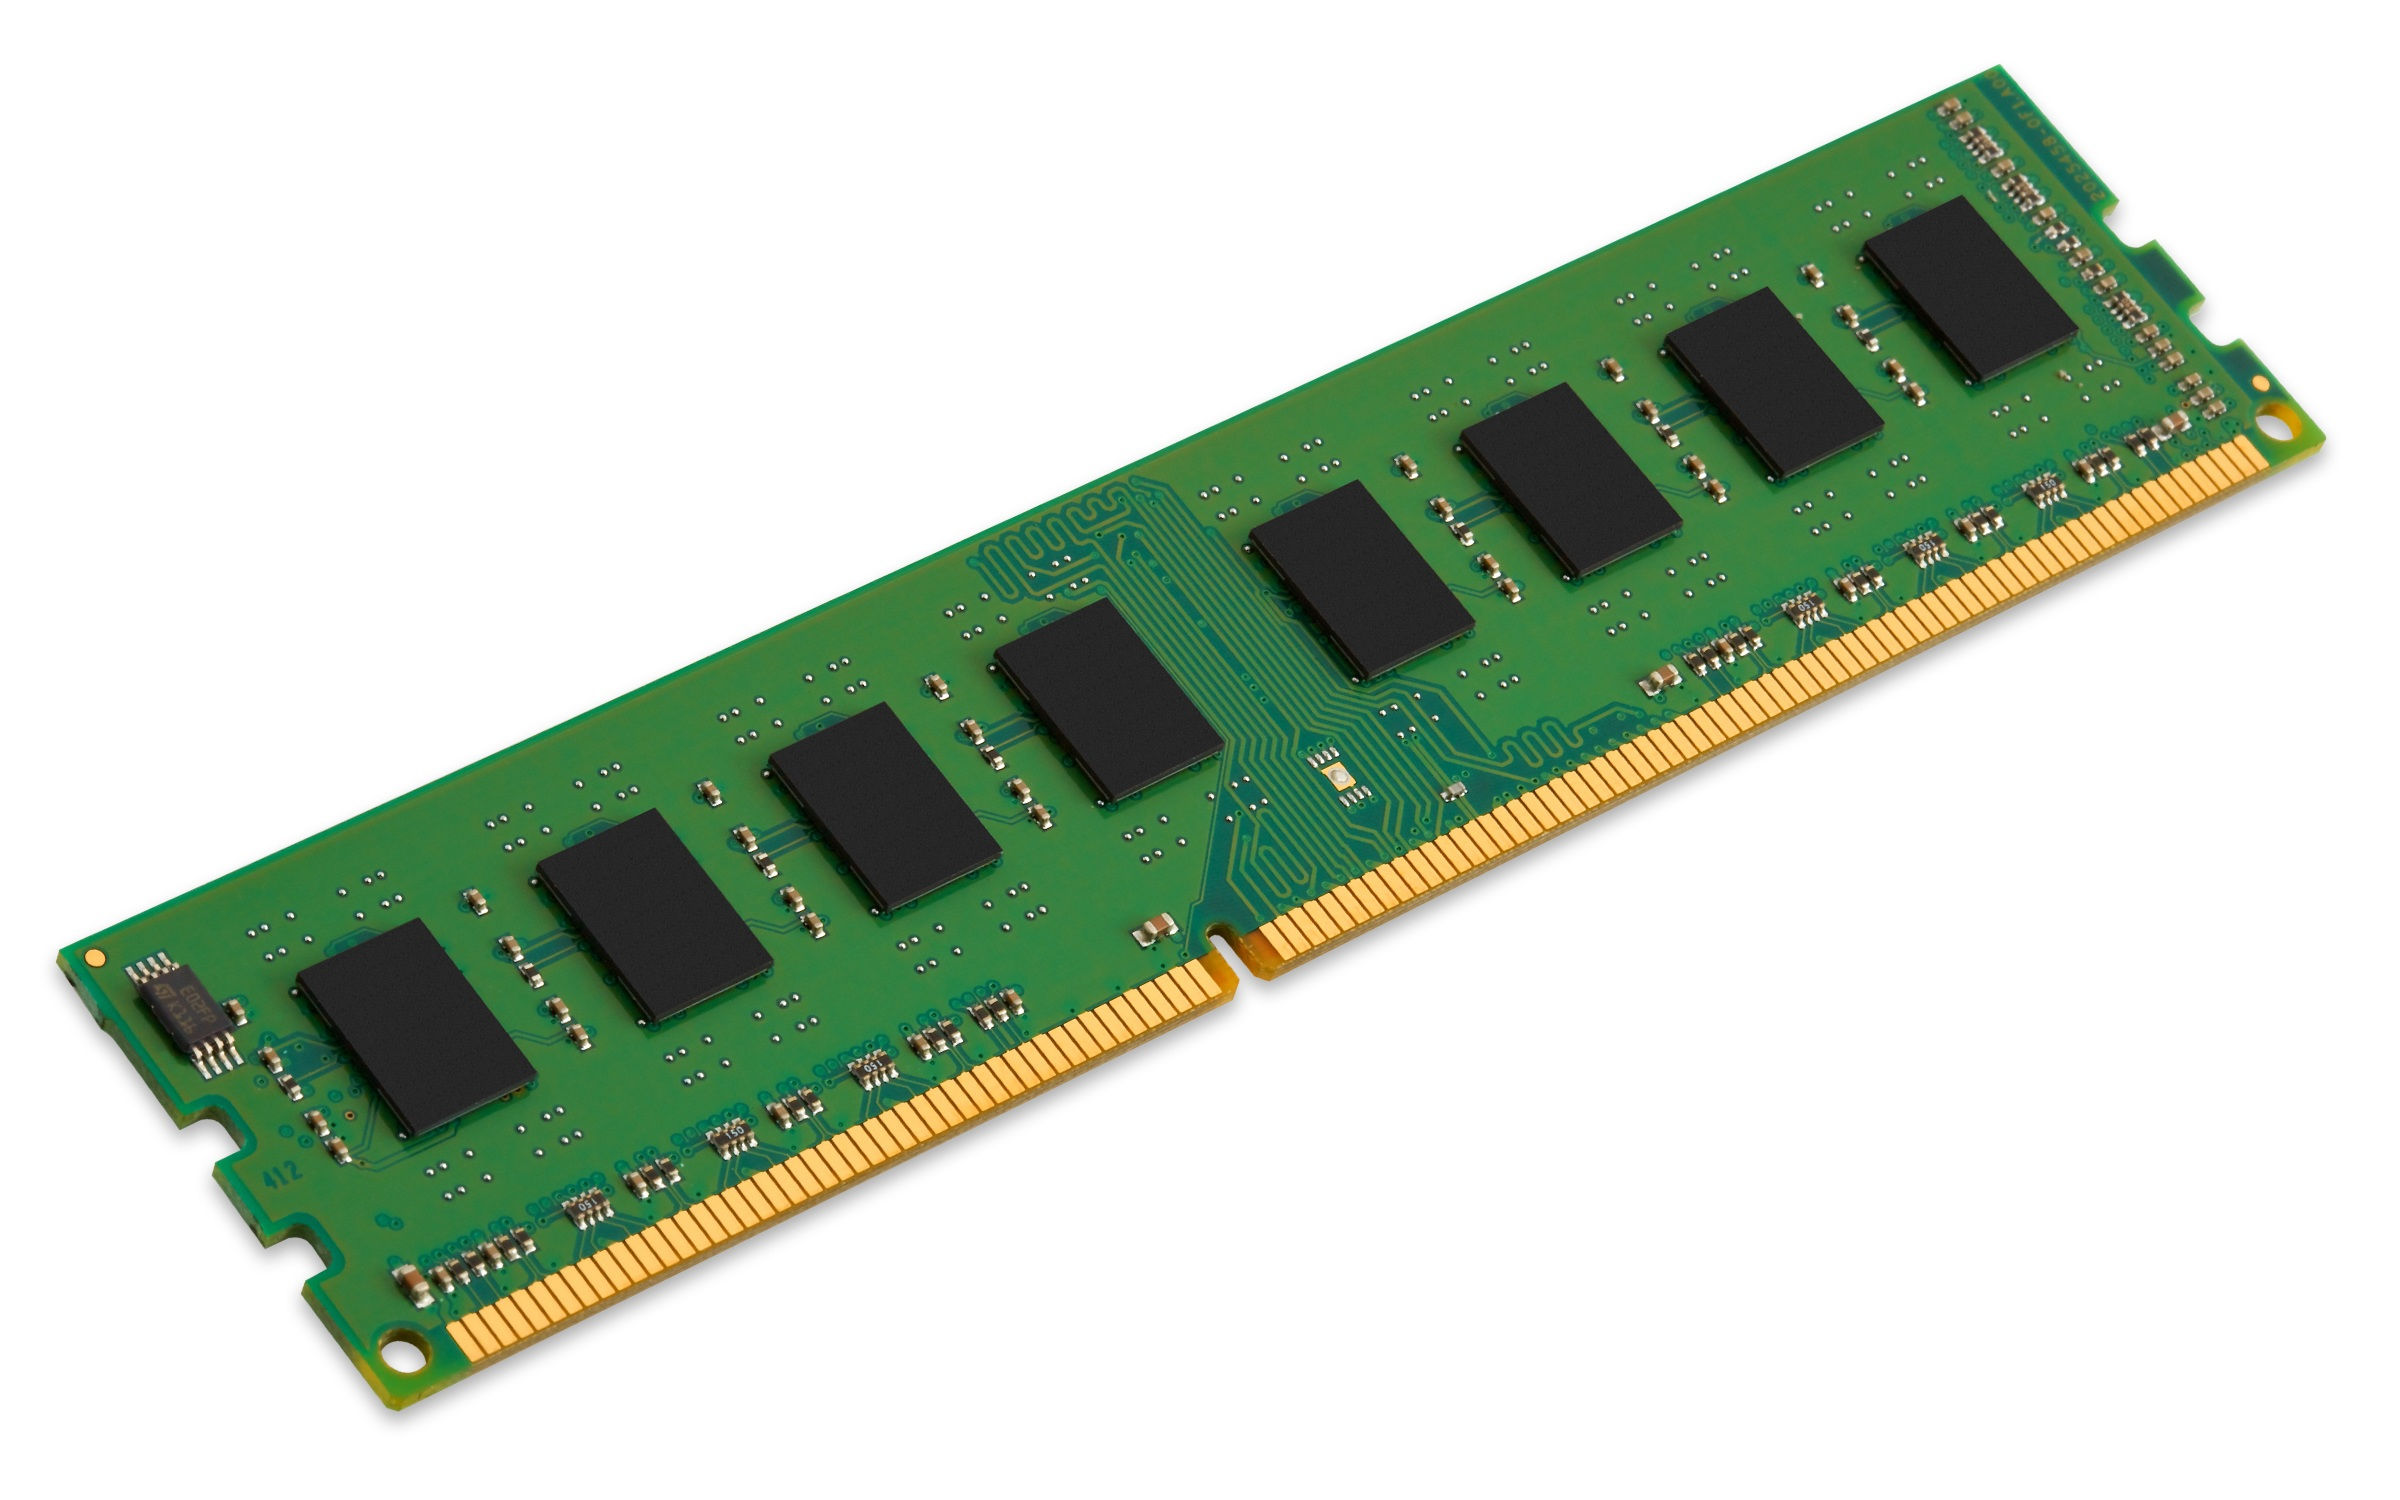
\includegraphics[scale=0.08]{img/ram.jpg}
        \caption{DIMM example}
        \label{fig:ram}
    \end{figure}
    
    \item Rank: This is a way to address the data in the DIMM, for example if we have x4 with 9 DRAMs per side you have the 36 bits. The controller has to access to 72 bits per transaction, so the when issuing a command reads or write both sides of the DIMM in that case the DIMM is single rank. If the DIMM is x8 then we have the 72 bits per side, so we only have to address one side. This is a dual rank, and we have to include in the address to which rank we are issuing the command.
    
    \begin{figure}
        \centering
        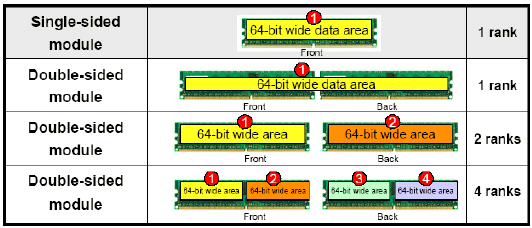
\includegraphics[scale=0.5]{img/dram_rank.png}
        \caption{DRAM rank examples}
        \label{fig:dram_rank}
    \end{figure}
    
    
    
    \item Chips in a bank: Each rank is composed by several chips. For example the x8 is composed by 8 chips per rank. Each one of those chips receive 1 byte of data, so for example if the data is 64 bits the first chip receive data[0:7],the second one data[8:15],... and the last one data[56:63]. 
    
    \item Banks: Each of the chips has banks which is a third dimension in the figure \ref{fig:dram_diag}. That means we have several repetition of the structure of rows and columns and in the address we have to select which one we want to read or write.
    \begin{figure}
        \centering
        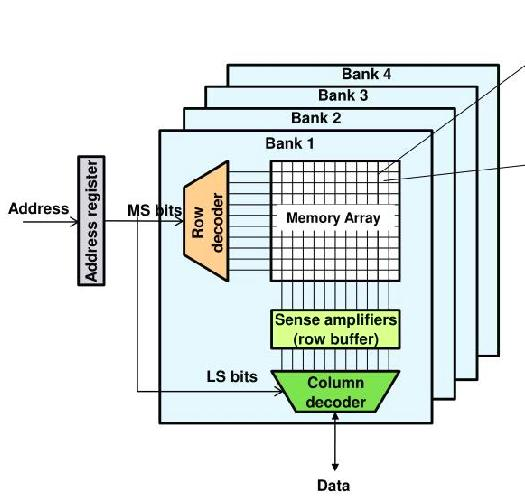
\includegraphics[scale=0.3]{img/dram_bank.jpg}
        \caption{Bank example}
        \label{fig:dram_bank}
    \end{figure}
    
    \item Finally we get into the row-column structure we first present.
    
\end{itemize}

After all that, the architecture could be summarize in figure 


\begin{figure}
    \centering
    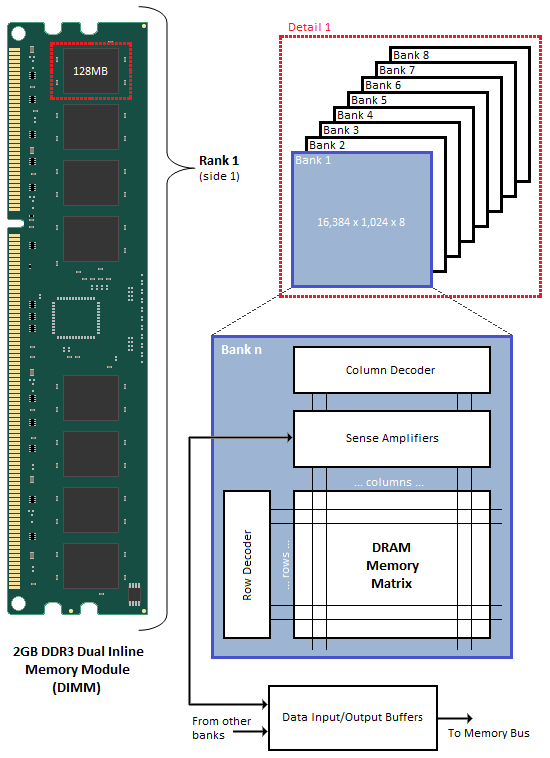
\includegraphics[scale=0.3]{img/dram_topology.png}
    \caption{DRAM topology.}
    \label{fig:dram_topo}
\end{figure}


In the memory interface generator you have to give as inputs, among other things, the target type of memory, the column, row and bank numbers, if the rank uses 8 or 9 bits (the 9th bit is for correction), etc.

\section{Signals}

Before starting is good to say that the DRAM uses a protocol with the differential signals standard in order to use both clock edges (that's why is called double rate). Usually the data is sent using several lanes at high data rate, when is received the data is parallelized to be process in a lower clock rate. For example a 2n prefetch means that internally the system is running at the half of the transfer rate but has a bus with the double size.
%\newp

Said that here are the main signals (to see all look at the \textbf{JEDEC STANDARD DDR3 SDRAM: JESD79-3C} ) as a notation the \# means the inverse signal:


\begin{itemize}
    \item CK, CK\#: clock signals.
    \item CKE: clock enable.
    \item CS: Chip select. This signal enables to select the rank if is not a single rank.
    \item RAS, CAS, WE: this signals names are an heritage from SRAM. Here define the type of command.
    \item DM: data mask. As its names suggest mask the valid data.
    \item BA0-BA2: Bank address input.
    \item A0-A15: Address input, in active command is the row address. In read/write commands is the column address.
    \item DQ: data input/output.
    \item DQS, DQS\#: data strobe.
\end{itemize}

 %\newp

The data strobes signals are bi directional signals that are emitted by the master of the bus, in the write mode is send by the controller (in our case the FPGA) in the read mode is send by the DRAM. It has three stages and are meant to be flags for the devices, like 
 ``brace yourself I'm coming with a bunch of data''.

\begin{itemize}
    \item Preamble: It's a time window where the sender gives a time windw for the receiver to get ready for the transfer.
    \item Toggling: When the data starts to be transfer the stroe starts to toggle between low and high at the clock frequency while the data burst last.
    \item Postamble: After the data burst is transfer there is a time window where the bus is in low.
\end{itemize}

There is a little (big) detail about this strobes signals. In read transaction is edge aligned with the data, so it changes are made in the rising edge of the bus clock. \textbf{BUT} for the write transaction this strobe signal are center aligned, which means that the strobe is running with $90^{\circ}$ phase difference with the data channel.


\begin{figure}
    \centering
    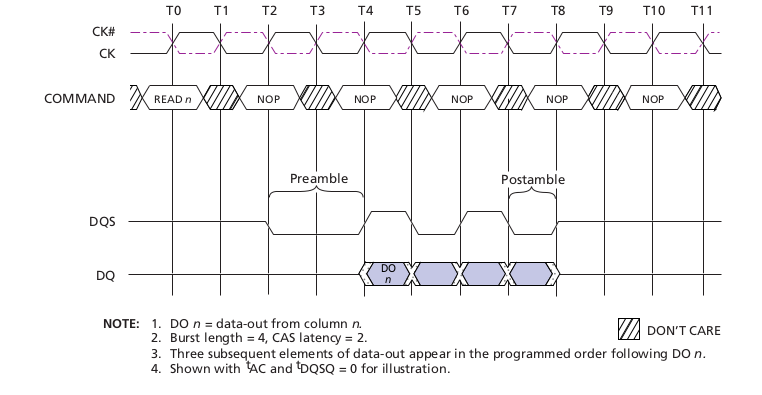
\includegraphics[scale=0.5]{img/read.png}
    \caption{Read transaction.}
    \label{fig:read}
\end{figure}


\begin{figure}
    \centering
    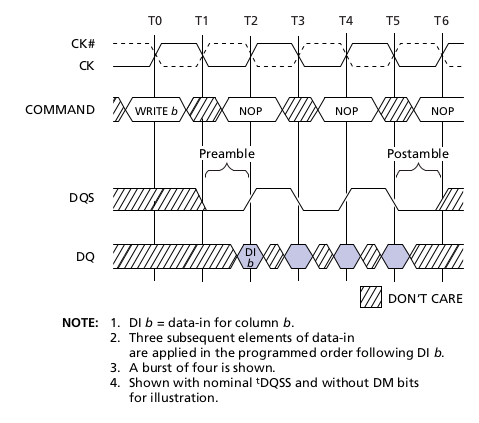
\includegraphics[width=12cm, height=8cm]{img/write.png}
    \caption{Write transaction.}
    \label{fig:write}
\end{figure}



\section{Xilinx solution}

Like you should be thinking the main problem here are the DQ, DQS signals. Because they change their phase with command that they are sending you can't get the signals with a simple PLL.
%\newp

Also the DRAMs runs at much higher frequency that the FPGA itself could handle. So we have to make a commitment, we cant get the standard with the usual re-configurable hardware so the solution is to use some dedicated hardware for that propose.
%\newp
In particular Xilinx uses Phasers wich are who generate the clocks with their correspondent reative phases, align the data also uses dome FIFOs to cross clock domains, order the data, etc.
And to send and receive the data use OSERDES and ISERDES. Where Serdes are Serialize-Deserialize logic that generates serial data running a higher clock rates from lower rate parallel inputs.

\begin{figure}
    \centering
    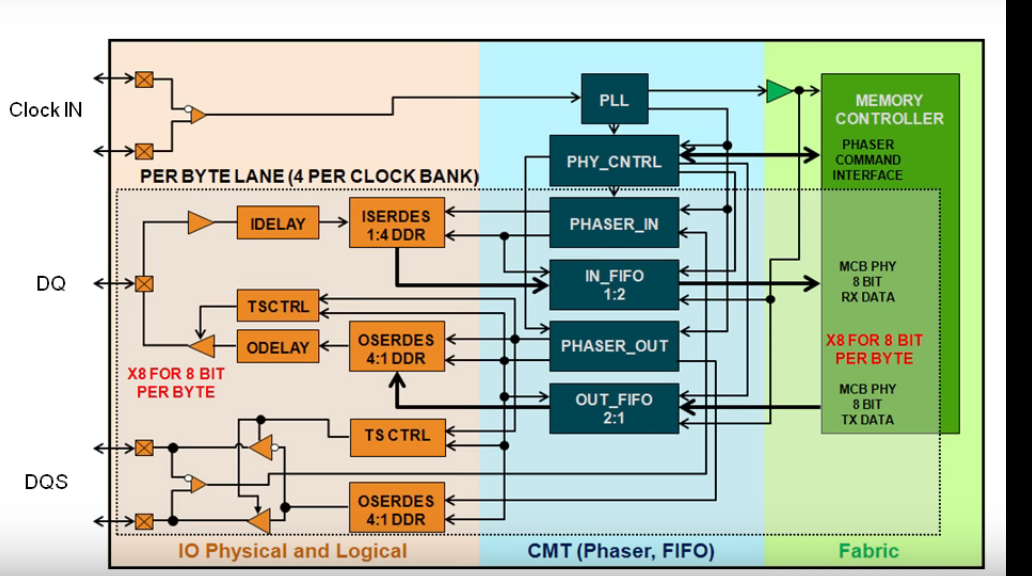
\includegraphics[scale=0.35]{img/mig_phy.png}
    \caption{MIG block design.}
    \label{fig:mig_phy}
\end{figure}


%\newp
Now we are entering to a dark place.. The physical interface that Xilinx give to us is really bad documented, if you want to use the IP directly there should be no problem but requires experience to program this things out of the IP.

For the DRAM we are fine because the DDR3 IP is free, but some times you would want to build your own interface to not paying for an IP but the physical part is not documented and you are stuck.. well that's life.


Besides the physical part (PHY) the Xilinx core generates a controller for the DRAM and get us a nice AXI interface so also hide the complexity of the addressing and other stuffs to the user. At the end you should be able to target the addresses of the DRAM in the same way you write a AXI slave.


\section{Using the Memory interface generator}

With all that we had present you should be ready to use the MIG to build a custom part. If you use a supported board you should have a default settings and just have to issue the block automation.

Here we present how to configure the MT8JSF25664HDZ for a kintex-420t. This a supported DRAM and has its default values, but we are going to configure it using a the custom options jut to show how to do it.

%\newp
The first 3 pages are straightforward, select \textbf{Create Design}, in the next page we select out device \textbf{xc7k420t-ffg90} and in the third page we mark the SDRAM3 controller.
%\newp

The fourth page is where we configure the settings for the DRAM that we are entering.

For the clock period we have to take a look to the supported speed of the DRAM that we are using and the supported frequency of the board.
The figure \ref{fig:dram_data_spedd} shows the speeds supported for the DRAM. The frequency supported by the kintex could be found in the \textbf{Kintex-7 FPGAs Data Sheet:DC and AC Switching Characteristics}.
\begin{figure}
    \centering
    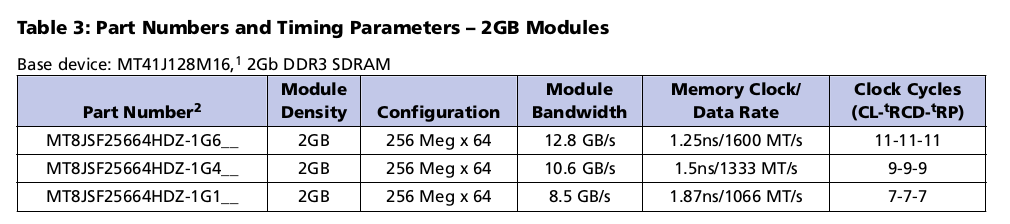
\includegraphics[scale=0.35]{img/dram_speed.png}
    \caption{ MT8JSF25664HDZ datasheet caption}
    \label{fig:dram_data_spedd}
\end{figure}

\begin{figure}
    \centering
    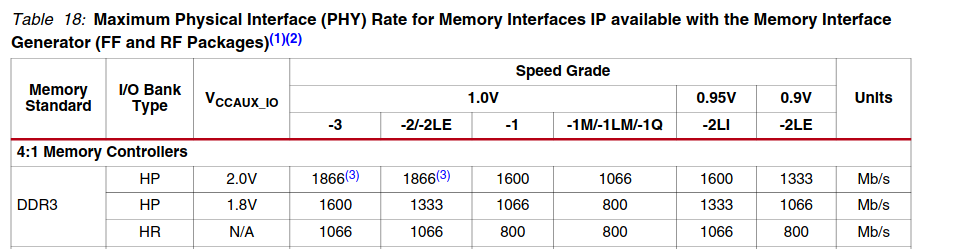
\includegraphics[scale=0.4]{img/kintex_speed.png}
    \caption{Kintex datasheet caption.}
    \label{fig:kintex_data}
\end{figure}

As you may think we are going to use the 1:4 memory controller which means that the controller is running at 1/4 of the PHY frequency.

With that in mind we set the clock rate in 1.875ps which is equivalent to 533.33MHz. This means that we are operating at 1066 MHz, which is supported by the both devices. (By the way here we use an HR IO bank, that's why the VCCaux its blocked).


%\newp
We set the memory type as \textbf{SODIMM} and then we click into the \textbf{Create Custom Part}.

This is going to open a new window where you have to fill the options with memory options. A tweak you need to know is that there is no visual option to select the rank, so if you are using a DRAM with double rank you have to select a double rank-DRAM as a base(I dont know if higher ranks are supported).
%\newp

\begin{figure}
    \centering
    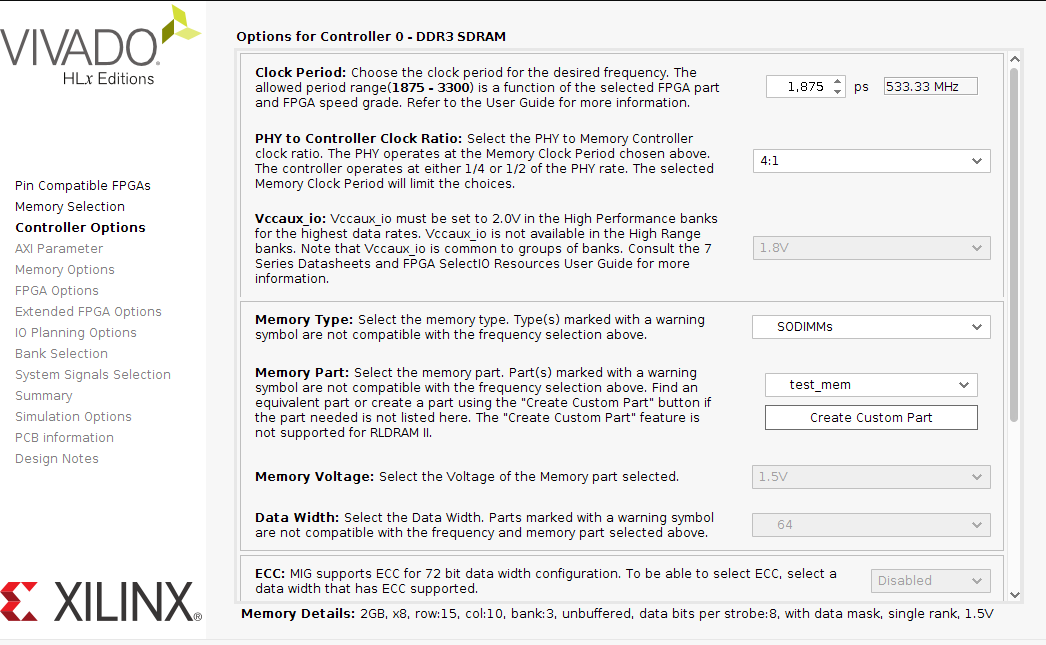
\includegraphics[scale=0.2]{img/mig_1.png}
    \caption{Controller options}
    \label{fig:mig_1}
\end{figure}

You have to look at the DRAM datasheet to search for the timing parameters, for example the table \ref{fig:timing} shows the trcd and trrd, but there are a lot of values missing in the datasheet :(. 
The official documentation of JEDEC has a large table with to calculate this parameters, but to have all the parameters you have to search for them across the entire document.

\begin{figure}
    \centering
    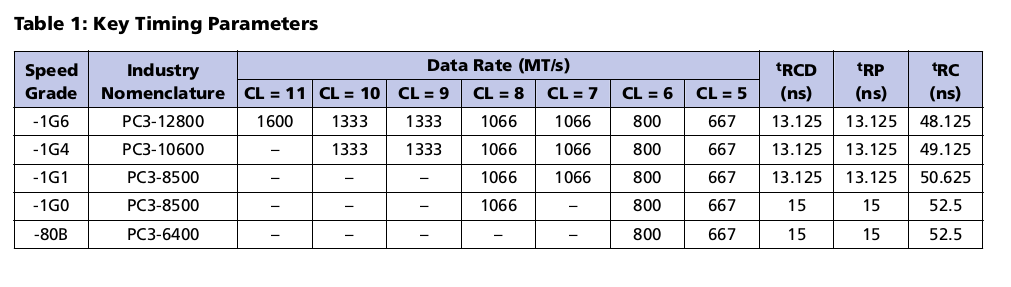
\includegraphics[scale=0.35]{img/timing_parameter.png}
    \caption{Some timing parameter}
    \label{fig:timing}
\end{figure}


%\newp 
I recommend using the templates of similar devices and use their default values and if the system doesn't works go back and modify this page. As we are using a supported device we are going to use the default time values that comes with this DRAM.
%\newp

The other important features are the bank, row, column numbers of your device. The MT8JSF25664HDZ addressing are shown in the figure \ref{fig:addrs}. So we have 15 row address, 10 column address and 3 bank address. In the last instance this values sets the size of the DRAM.

\begin{figure}
    \centering
    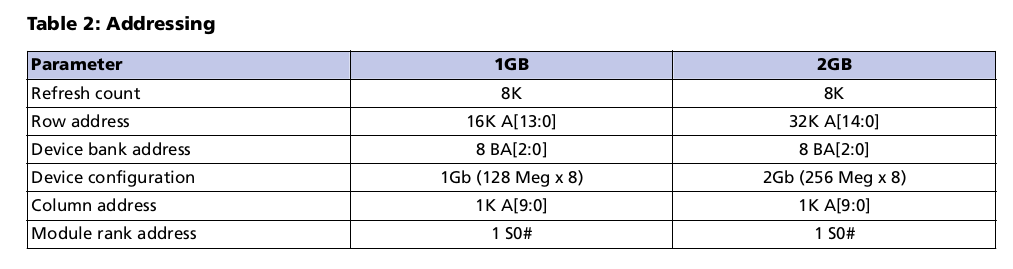
\includegraphics[scale=0.35]{img/dram_addr.png}
    \caption{MT8JSF25664HDZ addressing}
    \label{fig:addrs}
\end{figure}


You should check in the DRAM that the other values are right (for example your device has ECC ie it has 72 or 64 bits, or the rank is right?). Check the memory details in the bottom of the window.


The maximum value for the row address is 16 and for the column address is 11. With the 3 banks this give us 8GB, if you want to use a 16GB you have to use as template a dual rank memory. 

%\newp 
We keep the bank machines in 4 and the ordering in Normal.


The next window is the AXI parameters. Put here whatever you want, I put 512 because usually the DRAM has 8 length burst of 64bits, so we have a data burst of $64*8=512$, but you could use different numbers.

%\newp
In the next page, you need to give as input the FPGA clock that you are going to use to feed the MIG, in my case I set the value to 200MHz   because I have a 100MHz on board clock, so I only need to multiply it by two factor. 
Here you could also select if the MIG is going to generate output clocks for the use of the FPGA, we are not going to use them.


You could scroll a little bit in this page and set to set the termination status, you need to search for the right type in the DRAM datasheet. For our case we keep everything as default but you should check the impedance of your device before moving on.


You could also select to disable the Chip select (CS) which only make sense for the single rank devices. The idea is that if you are designing a FPGA you could save one pin, like we have a board with all the pins attached we don't care, we keep it enable.

The final option in this window is the memory addressing type that our DRAM has. To know that we need to look at the pin configuration in the DRAM datasheet, in specific the table in \ref{fig:addrs} tell us how the memory is addressed, the columns are first, followed by the rows and the banks are separated in a different signal group. We keep the default bank-row-column option. And click in the next button.


\begin{figure}
    \centering
    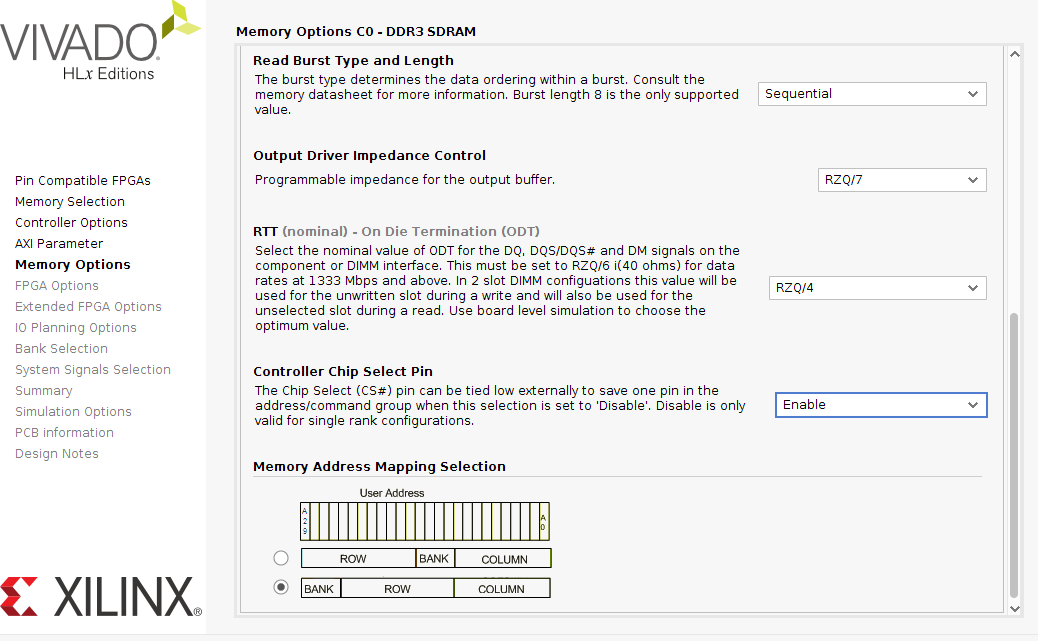
\includegraphics[scale=0.3]{img/mig_2.png}
    \caption{MIG memory options}
    \label{fig:mig_2}
\end{figure}


The next page are about how to clock the system, like we are going to use an internal clock we set the system clock without any buffer and in the reference clock we select to \textbf{Use system clock}.
Also we set the reset polarity to be active low, which is the typical standard.

We keep unmark the Internal Vref because our board already handles the powering of the devices externally. Also we keep the power reduction option and the XADC instantiation (allows correction due thermal variations). 

Click on next and now we set the internal impedance termination to be 50Ohm.
%\newp

In the IO planning we have two options, to make a new design and to use an existing one. Again, like our board has fixed the SODIMM interface we select the Fixed pin out option.
Now you have to map each pin with it correspondent task. The hard way to do it is to search for each pin in the schematic and map it to the each component, but your vendor should had gave you an xdc or ucf file with the pin assignment (some times its in the board files that you put in the Xilinx directory, if you dont have it Xilinx gaves a tempate of their chips, but you have to fill every pin with his right component).
You could upload a file with the assignment, but note that it needs to be feed with the exact name.


When you are ready press validate, if the engine doesnt complain press next.

\begin{figure}
    \centering
    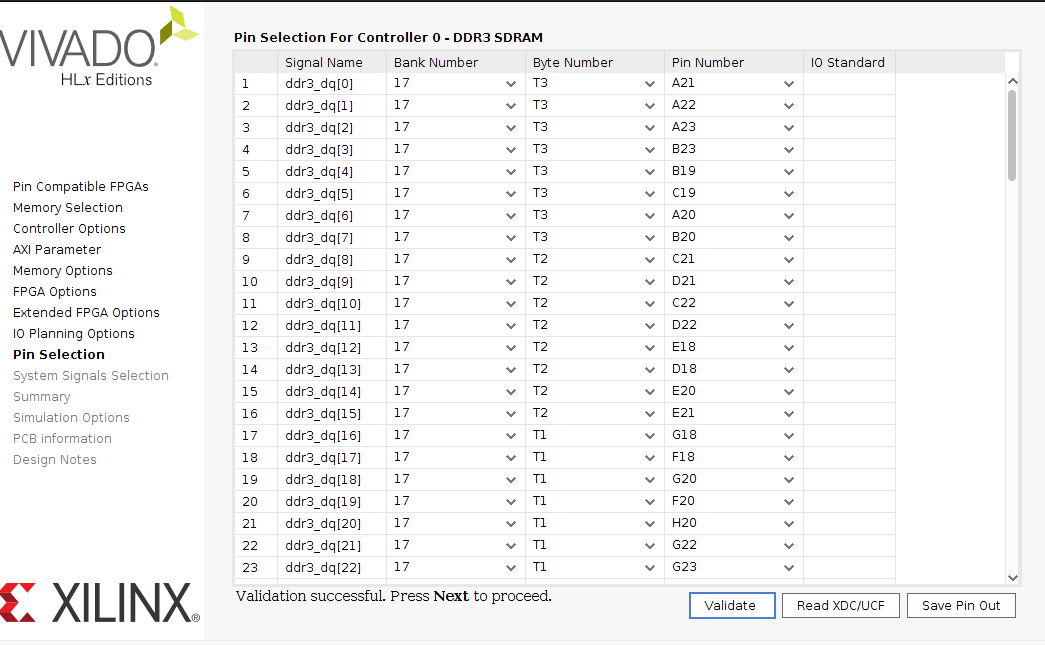
\includegraphics[scale=0.3]{img/mig_3.png}
    \caption{Pin selection.}
    \label{fig:mig3}
\end{figure}

The System signals page has some signals that could be connected into a pin or be internally driven by some FPGA logic.
We keep them unconnected.


\begin{figure}
    \centering
    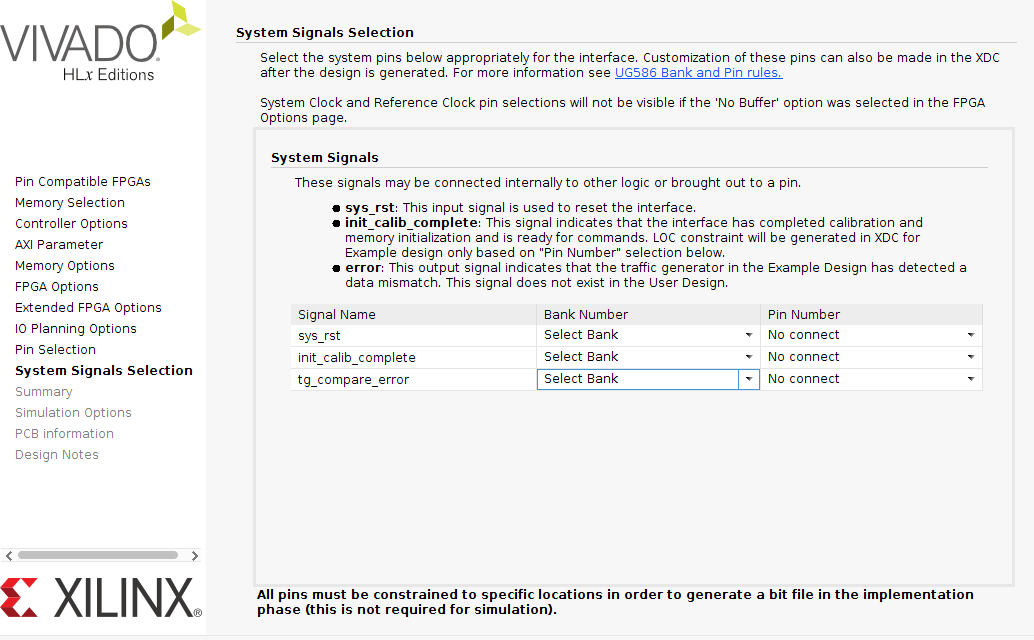
\includegraphics[scale=0.3]{img/mig_4.png}
    \caption{Signals selection}
    \label{fig:mig_4}
\end{figure}


Now we are almost ready, click next and a summary should appear. Is always good to take a look, when you are sure that everything looks good press next and keep pressing next until you see the generate button. Then and only then we are ready!

















































\begin{comment}

\section{Estado Red Pitaya data logger}


\subsection{Bus standar Xilinx}

La plataforma Red Pitaya esta basada en el SoC Zynq que a su vez esta compuesto de dos microprocesadores ARM más una FPGA. Al tener un procesador en el chip se pueden alcanzar altas tasas de trasnferencia entre el procesador y la FPGA con lo que el sistema esta diseñado para ser utilizado como sistema híbrido donde la FPGA y los procesadores trabajan de forma conjunta.

\begin{figure}
    \centering
    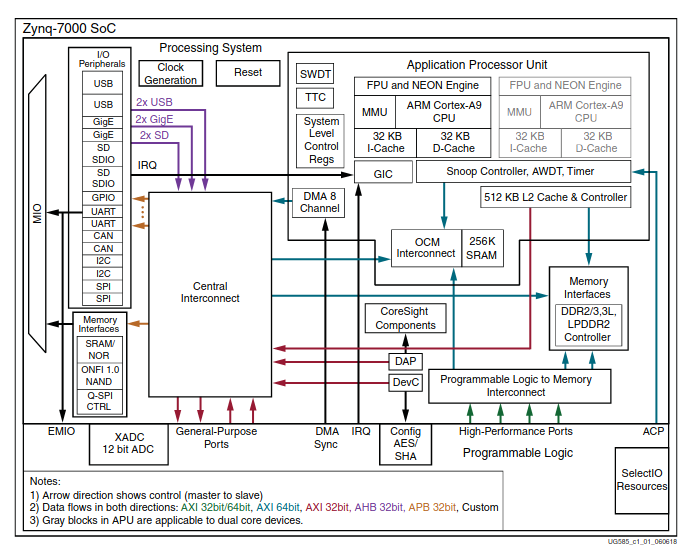
\includegraphics[scale=0.5]{img/ps.png}
    \caption{Diagrama del procesador dentro de Zynq}
    \label{fig:ps}
\end{figure}

Esto implica que debe existir un protocolo de comunicación entre la FPGA y el procesador, la solución soportada por Xilinx y por ARM es el bus AXI. 
El bus AXI consta de 3 sabores, AXI full, AXI lite y AXI stream. Como su nombre lo indica AXI stream es el protocolo utilizado por bloques que constantemente están stremeando datos, por ejemplo una FFT pipelined. AXI full genera un mapeo en memoria que escribe y lee utilizando burst diferentes tamaños, por ejemplo en una transacción puede escribir 256*4 bytes consecutivos en un AXI slave. AXI lite es una versión liviana de AXI full y permite escribir registros sin utilizar transacciones burst. 




En nuestro caso estamos interesados en utilizar AXI full para escribir a trozos la RAM dentro del procesador ARM. Esto puede lograrse de varias formas: 
\begin{itemize}
    \item Utilizar el IP de DMA de Xilinx.
    \item Crear la interfaz con el IP packager utilizando HDL.
    \item Crear la interfaz utilizando Vivado HLS.
    \item Utilizar la interfaz que viene en AXI master IPIC y ajustarse a sus entradas.
\end{itemize}


Actualmente tengo funcionando la opción del DMA con IP de Xilinx y la opción de crear la interfaz con HDL y soy capaz de escribir porciones de la memoria RAM del procesador con la FPGA y leerlas con el procesador.
Tambien tengo avanzado el wrapper para el IPIC y la interfaz hecha con HLS, pero no he podido implemntarlas en un modelo funcional. 


Algo que es deseable y que hasta este momento no se tiene completamente implementado es utilizar el DMA en scatter gatter mode. Esto es escribir en diferentes porciones de la memoria e ir moviendose de acuerdo a un patrón determinado.
Así por ejemplo en un primer burst puedes apuntar a escribir las direcciones 0x0000-0x1FFF, el segundo burst lo apuntas a 0x2000-0x3FFF, etc.
La gracia es que para el procesador es más fácil leer porciones que se encuentran una al lado de otra. Asi en vez de leer varias veces la posición 0x0000-0x2000, se puede leer una vez 0x000-0x4000 y además dar mas tiempo entre para el ciclo de trabajo del procesador.


\begin{figure}
    \centering
    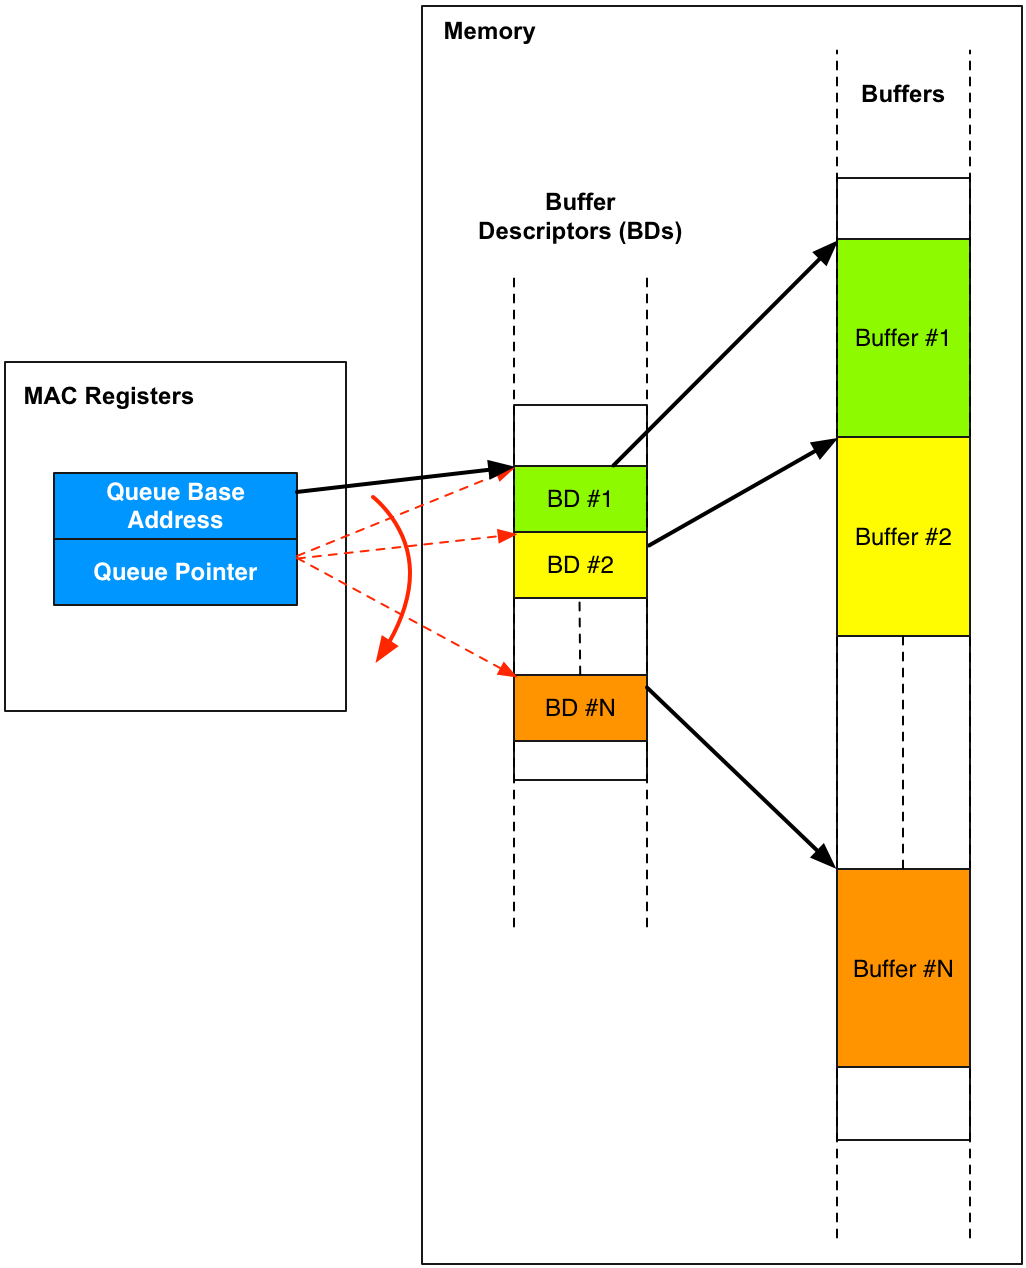
\includegraphics[scale=0.5]{img/scatter.png}
    \caption{Ejemplo de scatter Gather en un MAC, la idea en nuestro caso es similar.}
    \label{fig:scatter}
\end{figure}


Ambos modelos puede seleccionarse las direcciones ha escribir, pero esta no se ve actualizada dentro de la FPGA y es el procesador mediante un request quien debe entregar la dirección de destino en memoria. De todas formas ambas implementaciones pueden ser modificadas ligeramente para soportar scatter gather.

\subsection{Diagrama propuesto}

El diagrama de bloques propuesto para la parte de la FPGA puede verse en \ref{fig:diag}. La idea es la siguiente entran los datos por el ADC y pasan por un filtro CIC que es una implementación IIR de un promediador de manera que al reducir la frecuencia de muestreo se consideren las muestras eliminadas (notar que en este bloque quizás sea necesario conloca un filtro FIR compensatorio ya que la respuesta de un CIC permite cierto grado de aliasing).


\begin{figure}
    \centering
    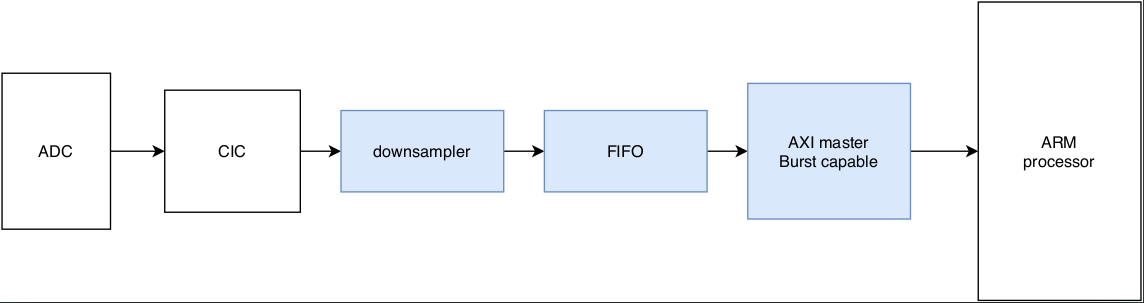
\includegraphics[scale=0.3]{img/diag.png}
    \caption{Diagrama propuesto}
    \label{fig:diag}
\end{figure}

El siguiente bloque es un \textit{downsampler} que no es nada mas que un descarte de muestras para tener una frecuencia de muestreo reducido.
Esto está implementado con un número de ciclos programable por el usuario.


Cada salida valida del downsampler va a un FIFO, cuando al interior del FIFO se juntan N muestras, donde N es el tamaño del paquete que se va ha enviar utilizando la interfaz AXI burst, se da la orden al AXI master de escribir la memoria. 
La implementación actual de este FIFO se escribe a $125MHz/downsampling$ y el AXI burst lee a $125MHz$ con lo que si se elige un tamaño de paquete y un downsampling adecuado el FIFO nunca debiese llenarse. Esto tiene otra limitante más que ha este momento no se ha medido, que es el numero de ciclos que toma enviar los datos por el AXI master. Pero por dar un ejemplo, si downsampleamos por un factor 10 y utilizamos un tamaño de paquete de 256, tenemos 2560 ciclos entre cada par de ciclos validos lo que debiese ser más que suficiente para enviar los datos.
Este FIFO con el conteo de datos en su interior también esta implementado.

El AXI master recibe el flag del FIFO de que el paquete ya se encuentra disponible, con lo que empieza a leer el FIFO y escribir la RAM. En estos momentos la dirección base puede se programada por el procesador, el tamaño del paquete es un parámetro harcoded que puede ser seteado al compilar el modelo.



Finalmente tenemos el procesador ARM donde hay varias salvedades. Hasta ahora no he realizado pruebas para medir el throughput que puede alcanzar el procesador, así como también es importante ver el ciclo de trabajo que se debe utilizar para la lectura de la RAM. Otra limitante en podría darse en la velocidad de escritura de un USB o de la SD, también sujeto a el tamaño de datos que se desee escribir en cada ciclo (ie acumular varias lecturas de la RAM y ahí recién escribir los datos en el storage device, otro motivo más para mirar scatter gather).


El ultimo ajuste que se debe observar en el procesador es que por default la red pitaya bootea en un linux OS y el kernel a priori utiliza todo el rango de las direcciones de la memoria. Aquí hay tres opciones:
\begin{itemize}
    \item Utilizar la Red Pitaya en modo bare metal. Ie sin OS, aquí tenemos toda las direcciones disponibles pero no tenemos algunos soportes, por ej hay que revisar como escribiir la SD o USB en este modo.
    \item Crear un Kernel custom. Podemos generar nuestra propia imagen y limitar el uso de la RAM por el Kernel y dejar el resto libre para el DMA.
    \item Utilizar la imagen de la red pitaya de Pavel Demin \url{http://pavel-demin.github.io/red-pitaya-notes/}. Esta imagen tiene libre la dirección $0x1E000000-0x40000000$. Pavel tambien tiene un modelo de recording de ADC, yo hasta ahora no he podido generar su modelo dentro de Vivado.
\end{itemize}

Personalmente me decantaría por la última opción, pero en el caso de necesitar aún mayor velocidad de lectura y escritura la opción de bare metal se vuelve más atractiva.



Un motivo para ir por el kernel custom es la posibilidad de trabajar con interrupciones en el sistema operativo. Se puede generar una señal de interrupción desde la FPGA hacia el procesador y trabajar la lectura de la RAM a nivel de kernel generando los drivers adecuados lo que también debiese mejorar la performance de lectura/escritura.


\end{comment}









\begin{comment}

\section{Sistemas con múltiples relojes}

Se les denomina sistemas con multiples relojes a aquellos sistemas digitales que poseen zonas que estan sincronizadas mediante relojes que corren a distintas frecuencias.

Existen 2 tipos de maneras de cambiar la frecuencia con que los datos pasan de un dominio de reloj a otro.
La primera consiste en hacer \textit{downsampling} y la segunda en hacer \textit{upsampling}. En este documento nos referiremos solo al \textit{Downsampling}.
\textit{Downsampling} consiste en descartar datos de manera que la cantidad de datos que pasen a la siguiente zona de reloj coincida con la frecuencia de dicha zona.


%\newp
Es decir si tenemos una señal $x[n]$ al realizar un \textit{downsampling} de factor M la señal resultante es $x[Mn]$ y descartamos el resto de las muestras tomadas.



%\newp

Por ejemplo, si tenemos un sistema con dos zonas de relojes donde la primera corre a a una frecuencia $f_{s}$ y la segunda zona corre a $f_{s}/2$ entonces es necesario hacer un \textit{downsampling} de orden 2, es decir de cada 2 datos descartamos uno y nos quedamos con el otro.

\insertimage[\label{img:downsampling}]{downsampling.png}{scale=0.4}{Ejemplo de Downsampling. a) Secuencia original b) Señal con un downsampling de factor 3}

%\newp
Se puede ver que el proceso de realizar un \textit{downsampling} por si solo no entrega ningún tipo de ganancia ya que estamos literalmente eliminando información.     

Y no solo eso, ya que al disminuir la frecuencia de muestreo del sistema podemos incurrir en un problema de aliasing.  


Ya que el ancho de banda de la primera zona es $B$ y el ancho de banda de la zona posterior a la reducción de frecuencia de muestreo es $B_{2} = B/M$, con lo que las frecuencias que en el ancho de banda original se encontraban sobre $B_{2}$ sufren de aliasing tras el \textit{downsampling} y caen dentro del nuevo ancho de banda.



%\newp
Es por ello que lo usual al hacer una reducción de frecuencia es colocar un filtro digital previo al \textit{downsampling}, así evadimos el problema del aliasing y dado que la característica de los filtros FIR o IIR consiste en sumar las entradas anteriores ponderadas por algún factor, cada dato que sale del filtro posee información de las muestras previas (en el caso de los FIR podemos considerar que la ventana temporal a la cual tiene acceso cada dato esta dado por el número de coeficientes del filtro).
Es decir, podemos pensar los filtros como una especie de promedio de las muestras en una ventana de tiempo dada para un determinado ancho de banda.

%\newp
A este combo filtro-\textit{downsampling} se le denomina decimación.

\insertimage[\label{img:decimacion}]{decimation.png}{scale=0.6}{Ejemplo de Decimación.}

\section{Oversampling}

La idea básica es reducir el ruido de cuantización de los ADC utilizando una  frecuencia de muestreo mayor a la requerida por el teorema de Nyquist.
%\newp
Esto parte de la suposición de que tenemos un ruido de cuantización que puede ser modelado como ruido blanco y por tanto su espectro es plano.
Con ello se tiene que la varianza del ruido total de cuantización está dado por \ref{eq:sigma_noise}
\begin{equation}
    \label{eq:sigma_noise}
    \sigma^{2} = \frac{(lsb Value)^{2}}{12}
\end{equation}

Con ello la densidad de potencia espectral de ruido esta dada por \ref{noise_PSD}.
\begin{equation}
    \label{noise_PSD}
    PSD_{noise} = \frac{(lsb Value)^{2}}{12f_{s}}
\end{equation}

Con \ref{noise_PSD} si aumentamos el valor de la frecuencia de muestreo podemos reducir el valor del ruido de cuantización.

%\newp
Dado que solo estamos interesados en una pequeña fracción del espectro podemos decimar y quedarnos solo con la zona de frecuencia que deseamos estudiar, y solo debemos preocuparnos que el filtro decimador posea la atenuación sufienciente para que el ruido no se meta en la banda base por aliasing.

\insertimage[\label{img:oversampling}]{oversampling.png}{scale=0.4}{Ejemplo de Oversampling.  a)PSD con la $f_{s}$    b)PSD con $f'_{s}$   c)Diagrama básico.}

%\newp
Ahora la ganancia que se genera al hacer oversampling esta dado por \ref{SNR} con respecto a muestrear con la frecuencia de Nyquist.



\begin{equation}
    \label{SNR}
    SNR_{improvement} = 10log(PSD_{fs}/PSD_{f'}) = 10log(f'/fs)
\end{equation}


%\newp
Tomando la expresión de \ref{SNR} y suponiendo que la nueva la frecuencia de oversampling $f'=fs*M$ y escribimos M convenientemente como $M=4^{r}$ tenemos que la mejora del SNR esta dada por $10log(M)=10log(4)*r \sim 6*r [dB]$. 
Con ello se suele mencionar que ganamos un bit cuando oversampleamos por una potencia de 4, haciendo referencia a la típica ecuación de SNR = 6.02N+1.76.

Aquí lo importante es que no ganamos bits por decimar, sino que por repartir el ruido de cuantización en un mayor ancho de banda al muestrear por una frecuencia mayor. 


\section{Diethering}

Diethering consiste en adicionar ruido analógico previo a la digitalización de manera que el bit menos significativo pueda ser excitado y por tanto supera el umbral del nivel de cuantización, generando variaciones en torno a dicho nivel. La idea es que las variaciones en torno al nivel tienen cierta tendencia dada por el valor real, con lo que podemos obtener un estimador del valor real si tomamos varias muestras de la variación y calculamos el valor promedio.

Por ejemplo si tenemos una señal con una amplitud de 0.8*lsb, al agregar ruido blanco podemos esperar que la proporción de veces que se excite el bit menos significativo con respecto al total de las mediciones debiese ser cercano al 80\% permitiendo determinar el valor de una señal bajo la resolución del ADC.


Es decir en este método ganamos información dado el comportamiento estadístico de los datos que al promediarlos podemos tener un estimador para un valor que se encuentra bajo la resolución típica del ADC y que mediante la adición de ruido se hace detectable.


%\newp
Cuando la señal de interés ocupa un lugar bien definido en el espectro se suele adicionar ruido de diethering con un nivel rms de 4 a 6 niveles de voltaje del lsb, lejos de la señal de interés y luego eliminarlo de manera digital.

%\newp
La ganancia de SNR seria proporcional $\sqrt{N}$, con N el numero de muestras que se están promediando. 

%\newp
Esto debido a que si el ruido es blanco, la componente de ruido al sumarse crece como $\sqrt{N}$ siguiendo la formula de random walk, mientras que al sumar señal con señal el valor crece como $N$.


%\newp
Con ello la mejora en SNR estaría dada por algo de la forma $SNR$ $\alpha$ $N/\sqrt{N} = \sqrt{N}$.


Nuestra idea es que el proceso de filtrado en la decimación es equivalente a calcular una especie de promedio sobre un ancho de banda dado con lo que estaríamos ganando resolución mediante la disminución de la frecuencia de muestreo.





\section{Que hacemos en el modelo que nos esta fallando}

Tenemos 3 etapas de decimacion, la primera con factor de decimación 16, la siguiente con factor 8 y la última con factor 4.
Por facilidad denotaremos las frecuencias de muestreo como $f_{1}$, $f_{2}$ y $f_{3}$ para cada zona de reloj. De igual forma los anchos de banda los denotaremos $B1$, $B2$ y $B3$. El diagrama del modelo puede verse en \ref{img:model}.


\insertimage[\label{img:model}]{model.png}{scale=0.4}{Diagrama del espectrómetro con factor de decimación 512.}


%\newp
En este caso el ADC está muestrando a 2160[MHz] y colocamos el primer filtro en la zona comprendida entre (0-70)MHz que es 1/16 de la frecuencia de muestreo de manera que coincida con el factor 16 de la decimacion. 
Con ello el ancho de banda de la primera decimacion es $B1=(0-67.5)[MHz]$.


%\newp
Dado que la señal que buscamos estudiar se encuentra en la zona de altas frecuencias de B1, buscamos utilizar el aliasing que se produce al hacer downsampling a nuestro favor. Con ello hacemos una especie de pass-band sampling digital en la zona de Nyquist en la que se encuentra la señal.

Con esto en mente colocamos el filtro de la segunda decimación en la banda comprendida en (50-60)[MHz] que corresponde a la 7 zona de Nyquist al hacer un downsampling de factor 8.



La idea es que el filtro pasa-banda elimina todas las componentes fuera de las frecuencias de interés y luego al realizar el downsampling la señal aparece replicada mediante aliasing en banda base. Un diagrama de lo que se hace se puede ver en \ref{img:bandpass}.



\insertimage[\label{img:bandpass}]{bandpass.png}{scale=0.4}{Ejemplo de decimación bandpass utilizando zonas de Nyquist para downconvertir la señal de interés a banda base.}


Con ello el ancho de banda de la señal tras la segunda decimación esta comprendida en (50.62-59.06)[MHz].

%\newp
La tercera etapa de decimación contiene un filtro pasabajo que corta en 52.5[MHz], y al tener un factor de decimación de 4 nos quedamos con un ancho de banda de 2.1093[MHz], comprendido entre (50.62- 52.73)[MHz].

%\newp

Este sistema en total tiene una decimación de factor 512 y tras ello se calcula un FFT de largo 1024, con lo que tenemos un espaciado de canal de 4.12KHz lo que seria equivalente a realizar una FFT de largo $2^{19}=524288$ sobre los datos que ingresan al ADC.



%\newp
La ultima respuesta que me dieron en el mailing list de CASPER es que puede ser que este teniendo un overflow en alguna etapa del modelo.


Esto dado que cuando estamos en un caso no favorable el piso de ruido sube aproximadamente 60dB, y lo que explican es que si tengo una muestra en la que ocurra un overflow produce un impulso de ruido cuya amplitud promedio sería 1/1000 y al repartir esta amplitud en todos los bins de la FFT tenemos que el ruido que ingresa a cada bin es 1/1000/1000 que serian los 60dB que estamos viendo. 
Así, tendríamos frecuencias para las cuales se esta produciendo un overflow que serian justamente las que se encuentran entre dos twiddle factors de la FFT.

%\newp
Aunque seleccioné las opciones de maximizar la precisión de cada bloque, dado que el crecimiento de los datos es demasiado alta en cada etapa, para mantener el tamaño de los datos manejabel corte el numero de bits y quizás la forma en que estoy manejando los rounding puede generar algún overflow.


El peor de los casos seria que exista un overflow dentro de la misma FFT. Ya que la FFT de Xilinx que estoy ocupando ya esta seteada con todos los parámetros para funcionar a su máxima precisión.

Dentro de la otra semana voy a revisar cada etapa por si es que en algún rounding estoy causando un overflow y ver si realizando shifts en la entrada de la FFT ayuda a evadir el problema.


\end{comment}






















